\documentclass[11pt]{scrartcl}
\usepackage{graphicx}
\graphicspath{{./}}
\usepackage[sexy]{evan}
\usepackage[normalem]{ulem}
\usepackage{hyperref}
\usepackage{mathtools}
\hypersetup{
    colorlinks=true,
    linkcolor=blue,
    filecolor=magenta,      
    urlcolor=cyan,
    pdfpagemode=FullScreen,
    }

\renewcommand{\dangle}{\measuredangle}

\renewcommand{\baselinestretch}{1.5}

\addtolength{\oddsidemargin}{-0.4in}
\addtolength{\evensidemargin}{-0.4in}
\addtolength{\textwidth}{0.8in}
% \addtolength{\topmargin}{-0.2in}
% \addtolength{\textheight}{1in} 


\setlength{\parindent}{0pt}

\usepackage{pgfplots}
\pgfplotsset{compat=1.15}
\usepackage{mathrsfs}
\usetikzlibrary{arrows}


\title{Symmedian dan Nine Point Circle - Homothety}
\author{Azzam (IG: haxuv.world)}
\date{Kamis, 15 Februari 2024}

\begin{document}
\maketitle
\renewcommand*\contentsname{Daftar Isi}
\tableofcontents
\newpage

\section{Materi}
\subsection{Symmedian}
\textbf{$A$-Symmedian adalah pencerminan dari garis berat dari $\angle A$ terhadap garis bagi $\angle A$}. Titik pertemuan dari tiga symmedian adalah titik symmedian (symmedian point).
\begin{figure}[h]
    \centering
    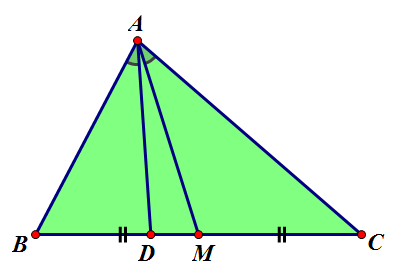
\includegraphics[scale=0.5]{Geometri/Symmedian-NinePoint/symmedian.png}
    \caption{Symmedian $AD$ dan median $AM$}
    \label{fig:symmedian}
\end{figure}
Pada gambar di atas, $AM$ adalah median atau garis berat dan $AD$ adalah $A-$symmedian dari $\triangle ABC$.

\subsubsection{Konstruksi Symmedian}
Misalkan $X$ adalah perpotongan dari garis singgung ke $ (ABC) $ di $ B $ dan $ C $. Maka garis $ AX $ adalah symmedian. (Pembuktiannya menjadi latihan soal)

\begin{figure}[h]
    \centering
    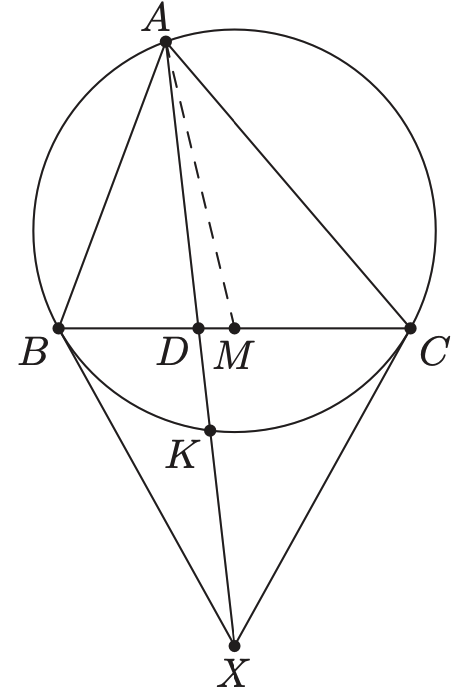
\includegraphics[scale=0.4]{Geometri/Symmedian-NinePoint/config_symmedian.png}
    \caption{Konstruksi Symmedian}
    \label{fig:symmedian-construction}
\end{figure}

\subsubsection{Properti dari Symmedian}
Misalkan $ ABC $ adalah segitiga, dan misalkan garis singgung ke lingkaran di $ B $ dan $ C $ bertemu di $ X $. Misalkan $ (ABC) $ memotong $ \overline{AX} $ di $ K $ dan $ BC $ di $ D $. Maka $ AD $ adalah $ A $-symmedian.
\begin{enumerate}[(a)]
\item $ KA$ adalah $K$-symmedian dari $ \triangle KBC $
\item $ \triangle ABK \sim \triangle AMC $.
\item
$ \frac{BD}{DC} = \left(\frac{AB}{AC}\right)^2 $
\item
$ \frac{AB}{BK} = \frac{AC}{CK} $
\item Lingkaran $ (BCX) $ melewati titik tengah dari $ AK $.
\item $ BC $ adalah $B$-symmedian dari $\triangle BAK$, dan $C$-symmedian dari $\triangle CAK$.
\item $BC$ adalah garis bagi dalam $\angle AMK$ dan $MX $ adalah garis bagi luar $\angle AMK$.
\end{enumerate}


\subsection{Nine Point Circle dan Homothety}
Nine point circle adalah salah satu konfigurasi geometri yang sangat bertumpu pada penggunaan teknik homothety (walaupun ya.... pakai kesebangunan biasa atau siklis juga bisa). Oleh karena itu, mari kita amati terlebih dahulu teknik homothety yang akan disajikan tersebut.

\subsubsection{Homothety atau Dilatasi}
Homothety atau dilatasi secara sederhananya adalah "perbesaran" atau "pengecilan" suatu bangun terhadap suatu titik pusat, sebutlah $O$ dan faktor skala $k$ (bisa positif atau negatif). Pada dasarnya ini adalah bentuk lain dari kesebangunan (namun dengan istilah yang keren :) )

Secara matematis, sebuah homothety $h$ adalah transformasi yang didefinisikan oleh titik pusat, sebutlah $O$, dan sebuah faktor skala bilangan real $k$. Homothety ini mengirim titik $P$ ke titik $h(P)$, dengan mengalikan jarak dari $O$ sebanyak $k$.

    \begin{figure}[h]
        \centering
        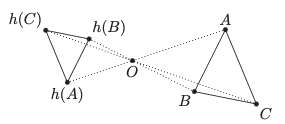
\includegraphics[scale=0.7]{Geometri/Symmedian-NinePoint/homothety-negatif.png}
        \caption{Homothety dengan pusat $O$ dan $k$ negatif}
        \label{fig:homothety-negatif}
    \end{figure}
    \begin{figure}[h]
        \centering
        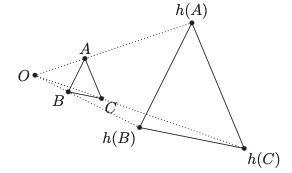
\includegraphics[scale=0.7]{Geometri/Symmedian-NinePoint/homothety-positif.png}
        \caption{Homothety dengan pusat $O$ dan $k$ positif}
        \label{fig:homothety-positif}
    \end{figure}

\begin{lemma}[Homothetic Triangle]
    \label{homothetic-triangle}
    Misalkan $ABC$ dan $XYZ$ adalah segitiga yang tidak kongruen sedemikian sehingga $AB \parallel XY$, $BC \parallel YZ$, dan $CA \parallel ZX$. Maka garis $AX$, $BY$, $CZ$ bertemu di suatu titik $O$, dan $O$ adalah pusat dari homothety $\triangle ABC$ ke $\triangle XYZ$.
\end{lemma}
\subsubsection{Nine Point Circle}
Akhirnya kita sampai ke konfigurasi utama dari materi homothety.
\begin{figure}[h]
    \centering
    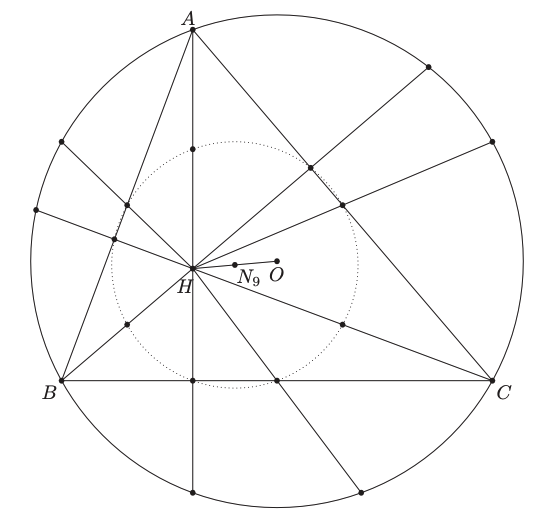
\includegraphics[scale=0.5]{Geometri/Symmedian-NinePoint/nine-point-circle.png}
    \caption{Nine Point Circle $\triangle ABC$}
    \label{fig:nine-point-circle-figure}
\end{figure}
\begin{lemma}[Nine Point Circle]
    \label{nine-point-circle}
    Misalkan $ABC$ adalah segitiga dengan pusat lingkaran $O$ dan titik tinggi (orthocenter) $H$, dan tandai $N_9$ sebagai titik tengah dari $OH$. Kemudian titik-tengah dari $AB$, $BC$, $CA$, $AH$, $BH$, $CH$, serta kaki tinggi dari $\triangle ABC$, berada pada lingkaran dengan pusat $N_9$. Selain itu, radius lingkaran ini adalah setengah dari radius $(ABC)$. Lingkaran ini adalah \textbf{nine point circle} dari $\triangle ABC$.
\end{lemma}


\section{Latihan Soal}
\subsection{Symmedian}
\begin{enumerate}
    \item Buktikan properti-properti symmedian di atas.
    \item Misalkan $X$ adalah perpotongan dari garis singgung ke $ (ABC) $ di $ B $ dan $ C $. Maka garis $ AX $ adalah symmedian.
    \item (OSP 2016) Misalkan $PA$ dan $PB$ adalah garis singgung lingkaran $\omega$ dari suatu titik $P$ di luar lingkaran. Misalkan $M$ adalah sembarang titik pada $AP$ dan $N$ adalah titik tengah $AB$. Perpanjangan $MN$ memotong $\omega$ di $C$ dengan $N$ di antara $M$ dan $C$. Misalkan $PC$ memotong $\omega$ di $D$ dan perpanjangan $ND$ memotong $PB$ di $Q$. Tunjukkan bahwa $MQ$ sejajar dengan $AB$.
    \item (Poland 2000) Let $ABC$ be a triangle with $AC = BC$, and $P$ a point inside the triangle such that $\angle PAB = \angle PBC$. If $M$ is the midpoint of $AB$, then show that $\angle APM + \angle BPC = 180^{\circ}$.

    \item (IMO Shortlist 2003) Three distinct points $A$, $B$, $C$ are fixed on a line in this order. Let $\Gamma$ be a circle passing through $A$ and $C$ whose center does not lie on the line $AC$. Denote by $P$ the intersection of the tangents to $\Gamma$ at $A$ and $C$. Suppose $\Gamma$ meets the segment $PB$ at $Q$. Prove that the intersection of the bisector of $\angle AQC$ and the line $AC$ does not depend on the choice of $\Gamma$.
    
    \item (Vietnam TST 2001) In the plane, two circles intersect at $A$ and $B$, and a common tangent intersects the circles at $P$ and $Q$. Let the tangents at $P$ and $Q$ to the circumcircle of triangle $APQ$ intersect at $S$, and let $H$ be the reflection of $B$ across the line $PQ$. Prove that the points $A$, $S$, and $H$ are collinear.
    
    \item (USA TST 2007) Triangle $ABC$ is inscribed in circle $\omega$. The tangent lines to $\omega$ at $B$ and $C$ meet at $T$. Point $S$ lies on ray $BC$ such that $AS \perp AT$. Points $B_1$ and $C_1$ lies on ray $ST$ (with $C_1$ in between $B_1$ and $S$) such that $B_1T = BT = C_1T$. Prove that triangles $ABC$ and $AB_1C_1$ are similar to each other.
    
    \item (USA 2008) Let $ABC$ be an acute, scalene triangle, and let $M$, $N$, and $P$ be the midpoints of $BC$, $CA$, and $AB$, respectively. Let the perpendicular bisectors of $AB$ and $AC$ intersect ray $AM$ in points $D$ and $E$ respectively, and let lines $BD$ and $CE$ intersect in point $F$, inside of triangle $ABC$. Prove that points $A$, $N$, $F$, and $P$ all lie on one circle.
\end{enumerate}



\subsection{Nine Point Circle dan Homothety}
\begin{enumerate}[resume]
    \item Buktikan lemma homothetic triangle \ref{homothetic-triangle}.
    \item Buktikan lemma nine point circle \ref{nine-point-circle}.
    \item Buktikan bahwa titik berat (centroid) segitiga membagi median (garis berat) dengan rasio $2:1$.
    \item (Euler Line) Pada segitiga $ABC$, misalkan $O,G,H$, dan $N_9$ berturut-turut adalah circumcenter, centroid, orthocenter, dan nine point center dari $\triangle ABC$. Buktikan $O,G,H, N_9$ kolinear dan $G$ membagi $OH$ dalam rasio $2:1$.
    \begin{figure}[h]
        \centering
        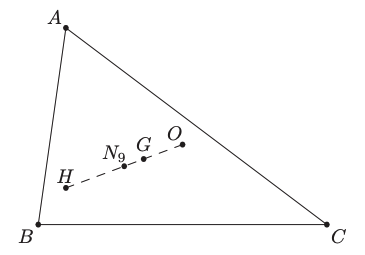
\includegraphics[scale=0.4]{Geometri/Symmedian-NinePoint/euler-line.png}
        \caption{Euler Line}
        \label{fig:euler-line}
    \end{figure}
    \item (OSN 2022) Pada segitiga $ABC$, titik $D$ dan $E$ berada pada sisi $AB$ dan $AC$ berturut-turut sehingga $DE$ sejajar dengan $BC$. Diketahui bahwa terdapat titik $P$ pada interior segiempat $BDEC$ sehingga $\angle BPD = \angle CPE = 90^{\circ}$. Buktikan bahwa garis $AP$ melalui titik pusat lingkaran luar dari segitiga-segitiga $EPD$ dan $BPC$.
    \item (OSN 2018) Misalkan $\Gamma_1$ dan $\Gamma_2$ adalah dua lingkaran yang bersinggungan di titik $A$ dengan $\Gamma_2$ di dalam $\Gamma_1$. Misalkan $B$ adalah titik pada $\Gamma_2$ dan garis $AB$ memotong $\Gamma_1$ di titik $C$. Misalkan $D$ adalah titik pada $\Gamma_1$ dan $P$ adalah titik sembarang pada garis $CD$ (titik ini bisa berada pada perpanjangan segmen $CD$). Garis $BP$ memotong $\Gamma_2$ di titik $Q$. Tunjukkan bahwa $A$, $D$, $P$, dan $Q$ terletak pada satu lingkaran.
    \item (BAMO 2013) Let $H$ be the orthocenter of an acute triangle $ABC$. Consider the circumcenters of triangles $ABH$, $BCH$, and $CAH$. Prove that they are the vertices of a triangle that is congruent to $ABC$.
    \item (USAMO 1993) Let $ABCD$ be a quadrilateral whose diagonals $AC$ and $BD$ are perpendicular and intersect at $E$. Prove that the reflections of $E$ across $AB$, $BC$, $CD$, $DA$ are concyclic.
    \item (EGMO 2013) The side $BC$ of the triangle $ABC$ is extended beyond $C$ to $D$ so that $CD= BC$. The side $CA$ is extended beyond $A$ to $E$ so that $AE= 2CA$. Prove that if $AD= BE$ then the triangle $ABC$ is right-angled.
\end{enumerate}
\section{Referensi}
\begin{itemize}
    \item Evan Chen, Euclidean Geometry on Mathematical Olympiad, MAA Press, 2016.
    \item \url{https://brilliant.org/wiki/symmedian/}
    \item Yufei Zhao, Lemmas in Euclidean Geometry, \url{https://web.mit.edu/yufeiz/www/olympiad/geolemmas.pdf}
\end{itemize}
\end{document}
